\chapter{Annotation Service}

\section{Objective of the Annotation Service}
\label{sec4_objective}
As described in \ref{sec2_as}, the goal of the AS is to provide a user with the possibility to:
\begin{enumerate}[(1)]
	\item view A WSI
	\item annotate a WSI
	\item manage made annotations
\end{enumerate}

In order to achieve objective (1) - (3), a GUI needs to be deployed which supports the user in working on those tasks. (3) also adds the need for file persistence management.

It became clear during the development process that the support of only DZI was impractical for the real life environment of the AS, thus making it necessary to support proprietary formats as well. A solution has to be found, that still addresses the vendor and platform issues stated in \ref{sec1_researchObjective} and \ref{sec2_openFormats}.


\section{Methodology}
\label{sec4_methodology}
As stated in \ref{sec2_openFormats}, most vendors have proprietary image formats and their own implementation of a viewer for those, thus creating a vendor lock-in. Further do vendors often support only Windows platforms, ignoring other operating systems\cite{Cornish13},\cite{DICOM10},\cite{Farahanil15}. To avoid this, a solution must be found that is independent of operating system and vendor.

Independence from an operating system can be achieved by using web technologies, especially when running an application in a web browser, since those are supported by all modern operating systems and even mobile platforms\cite{Tseytlin14}.

To develop the AS as a web application means to become subject to \emph{cross-origin resource sharing} (CORS)\nmc{CORS}{Cross Origin Resource Sharing}\cite{Kesteren14} and the \emph{same-origin policy} (SOP)\cite{web:mdn}\nmc{SOP}{Same-Origin Policy}. The SOP is a security concept of the web application security model, that only allows direct file access if the parent directory of the originating file is an ancestor directory of the target file\cite{web:mdn}. Since the local WSI file will not have the same origin, CORS is needed. CORS is a standard that defines mechanisms to allow access to restricted resources from a domain outside of the origin, when using the HTTP protocol\cite{Kesteren14}. Since the WSI is a local file, HTTP can not be used to retrieve the file.

The restrictions of SOP and CORS can be worked around by deploying a server as so called \emph{digital slide repository} (DSR). A DSR manages storage of WSIs and their metadata\cite{Cornish13}. This way, WSIs would share the same origin as the viewer and their retrieval would be possible.

Using a DSR has additional advantages: 
\begin{itemize}
	\item WSIs are medical images and as such confidential information. Their access is usually tied to non-disclosure or confidentiality agreements (e.g. \cite{COA} or \cite{USSanDiego}). A DSR eliminates the need to hand out copies of WSIs, which makes it easier to uphold the mentioned agreements.
	\item WSIs take up big portions of storage\cite{Singh11}. The local systems used by pathologists in the environment of the AS are usual desktop computers and laptops. As such, their storage might be insufficient to hold data in those quantities. A DSR can be set up as a dedicated file server, equipped for the purpose of offering large amounts of storage.
	\item A DSR enables centralized file management. Pathologists don't access local their local version of a WSI and it's annotations, but share the same data pool.
	\item Depending on the network setup, other advantages become possible, e.g. sharing of rare cases as educational material and teleconsultation of experts independent of their physical position\cite{Wilbur09}.
\end{itemize}

Chapter \ref{sec3_cs} established a service to convert WSIs of various, proprietary formats to DZI, addressing the need to implement multiple image format drivers. But, as stated in \ref{sec4_objective}, a solution to serve proprietary image formats without explicit conversion must be found.

\emph{OpenSlides Python} provides a DZI wrapper. This wrapper can be used to wrap a proprietary WSI and treat it as a DZI\cite{web:openslide}. A DSR can use this to serve a proprietary WSI as DZI to a viewer.

For the reasons mentioned above, the AS will be implemented as a web application. To do so, it will be split into 2 parts: a DSR and a viewer.


\section{Parts of the Annotation Service}
\label{sec4_parts}
As described in section \ref{sec4_methodology}, the AS will be realized in 2 separate parts:
\begin{itemize}
	\item a DSR, called \emph{Annotation Service Server} (ASS)\footnote{
		ASS is pronounced "A2S".
	}\nmc{ASS}{Annoation Service Server} (see subsection \ref{sec4_assPart})
	\item a viewer, called \emph{Annotation Service Viewer} (ASV)\nmc{ASV}{Annotation Service Viewer} (see subsection \ref{sec4_asvPart})
\end{itemize}

The ASS will be responsible for data management, supplying image data and serving the ASV to the client. The ASV will provide a WSI viewer with the tools needed to annotate ROIs in a WSI.

The two components interact as follows: once the client requested a valid image URL, the ASS will check if the requested WSI is a DZI and, if so, render a ASV with the image path, MPP and file name of the WSI. If the WSI is proprietary, it will be wrapped by OpenSlide. The remaining procedure is then identical to the DZI case.

The ASV is returned to the client and requests the data necessary to view the WSI and it's annotation if they should already exist (this includes configurations, annotations, labels and the image tiles for the current view).

Once loaded, the client can change the current view to maneuver through the different levels and image tiles available, which will be requested by the ASS whenever needed. Additionally, annotations can be made and persisted at any time.

See fig. \ref{fig4_asUml} for a diagram of how the ASS and ASV interact with each other.

\begin{figure}[!h]
	\begin{center}
		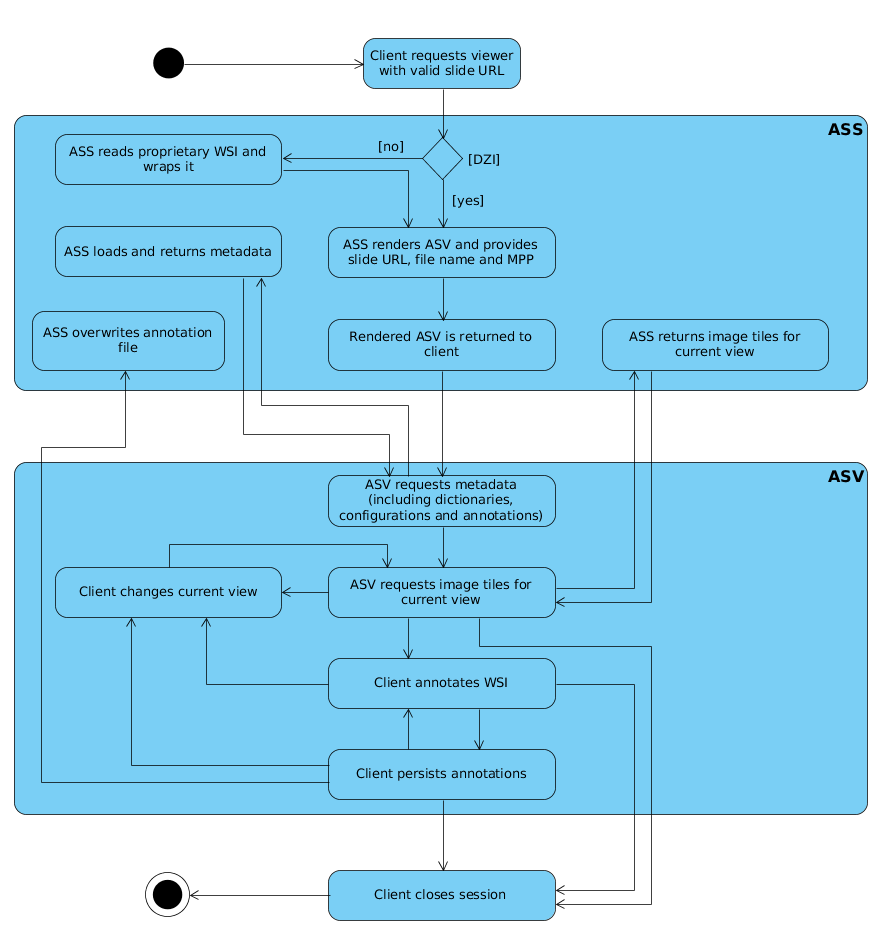
\includegraphics[scale=0.4]{img/asUML.png}
		\caption{Activity diagram of ASS and ASV}
		\label{fig4_asUml}
	\end{center}
\end{figure}


\subsection{Annotation Service Server}
\label{sec4_assPart}
As described in section \ref{sec4_methodology}, the ASS serves as a DZR. As such it is responsible for the storage of WSI files and their related metadata\cite{Cornish13}. Additional data managed by the ASS will be:

\begin{itemize}
	\item annotation data
	\item the ASV's configuration data
	\item dictionary data
\end{itemize}

Communication with the ASS directly is only necessary to request the rendering of an ASV with a WSI. Once the ASV is rendered, communication can be handled through shortcuts in the ASV.\clearpage

Communication between ASS and client, as well as ASS and ASV, will be realized over a RESTful API\footnote{
	\emph{Representational State Transfer} (REST)\nmc{REST}{Representational State Transfer} is an architectural style for developing web applications. It was established in 2000 by Fielding in \cite{Fielding00}. A system that complies to the constraints of REST can be called RESTful. Typically, RESTful systems communicate via the HTTP protocol\cite{Fielding00}.
	} offered by the ASS.

The development of a fully functional web server is not within the scope of this thesis. Therefore, the ASS will run as a local web server. This works around many of the common issues when hosting a web server (e.g. inefficient caching, load balance issues, gateway issues, poor security design, connectivity issues)\cite{web:typicalissues}.


\subsection{Annotation Service Viewer}
\label{sec4_asvPart}

The ASV is developed to provide a WSI viewer with annotation capabilities. It serves as main component for interaction with the AS, realizing most of the communication with the ASS (compare fig. \ref{fig4_asUml}).

The annotation capabilities look as follows:
\begin{itemize}
	\item Annotations will be represented by so called \emph{regions}. A region is defined by a path enclosing the ROI. This path can be drawn directly onto the WSI. The drawing is done either in \emph{free hand} or \emph{polygon} mode. When drawing free hand, the path will follow the mouse cursor along its way as long as the drawing mode is activated. In polygon mode, segments can be placed, which are connected with a path in the order that they were placed in.
	
	\item Each region has an associated \emph{label} that describes the region. A label is a keyword, predefined by a \emph{dictionary}. A dictionary contains a list of keywords that are available as labels.
	
	\item New, empty label dictionaries can be created.
	
	\item New labels can be added to existing dictionaries.
	
	\item Each region has a \emph{context} trait. This trait lists all other regions that
	\begin{itemize}
		\item touch
		\item cross
		\item surround
		\item are surrounded by
	\end{itemize}
	the region (see fig. \ref{fig4_contextregions}).

	\item A \emph{point of interest} (POI)\nmc{POI}{Point of Interest} is another way to create a region. After selecting a POI (a point coordinate in the image), an external script will start a segmentation\footnote{
		Segmentation approaches differ drastically between cases and scenarios\cite{Liu12}, see e.g. \cite{Qi12}, \cite{Sharma16}, \cite{Wienert12} or \cite{Angulo10} alone for cell segmentation. Since image segmentation exceeds the scope of this work by far, only a dummy implementation will be delivered, to show basic functionality. The script will be an interchangeable python plug in.
	} and return the image coordinates for an enclosing path to the ASV. The ASV will then automatically create a region based on the provided information.
	
	\item For annotation support, a distance measurement tool is provided. This tool can measure the distance between 2 pixels in a straight line\footnote{
		The measurement will be realized by the euclidean distance between a pixel $p_A$ and $p_B$\cite{Strang03}.
	}	
\end{itemize}

\begin{figure}[H]
	\begin{center}
		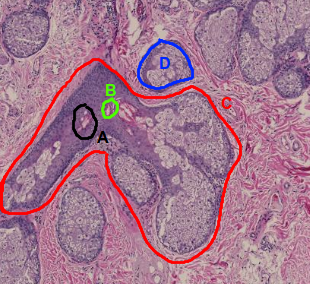
\includegraphics[scale=0.55]{img/contextregions.png}
		\caption{Example of context regions (B, C are context of A; A, C are context of B; A, B are context of C; D has no context region)}
		\label{fig4_contextregions}
	\end{center}
\end{figure}

The ASV uses keywords from a dictionary to label regions. While a free text approach is more flexible and easier to handle for novice users, it encounters difficulties in a professional metadata environment (such as histopathological image annotation). A dictionary-based approach facilitates interoperability between different persons and annotation precision\cite{Frosterus11}. To increase flexibility, the ASV will offer the possibility of adding new entries to existing dictionaries.

Since the vocabulary may vary strongly between different studies, the ASV offers the possibility to create new dictionaries. This way, dictionaries can be filled with a few case-relevant keywords instead of many generic, mostly irrelevant ones\footnote{
	This does not exclude the use of a "generic" dictionary if it should serve a broad series of cases.
}.

The first iteration of the ASV will be based on an open source project called \emph{MicroDraw}\footnote{See \url{https://github.com/r03ert0/microdraw} for more information on the MicroDraw project} (see fig. \ref{fig4_microdrawUI} for MicroDraw's GUI).  

\begin{figure}[H]
	\begin{center}
		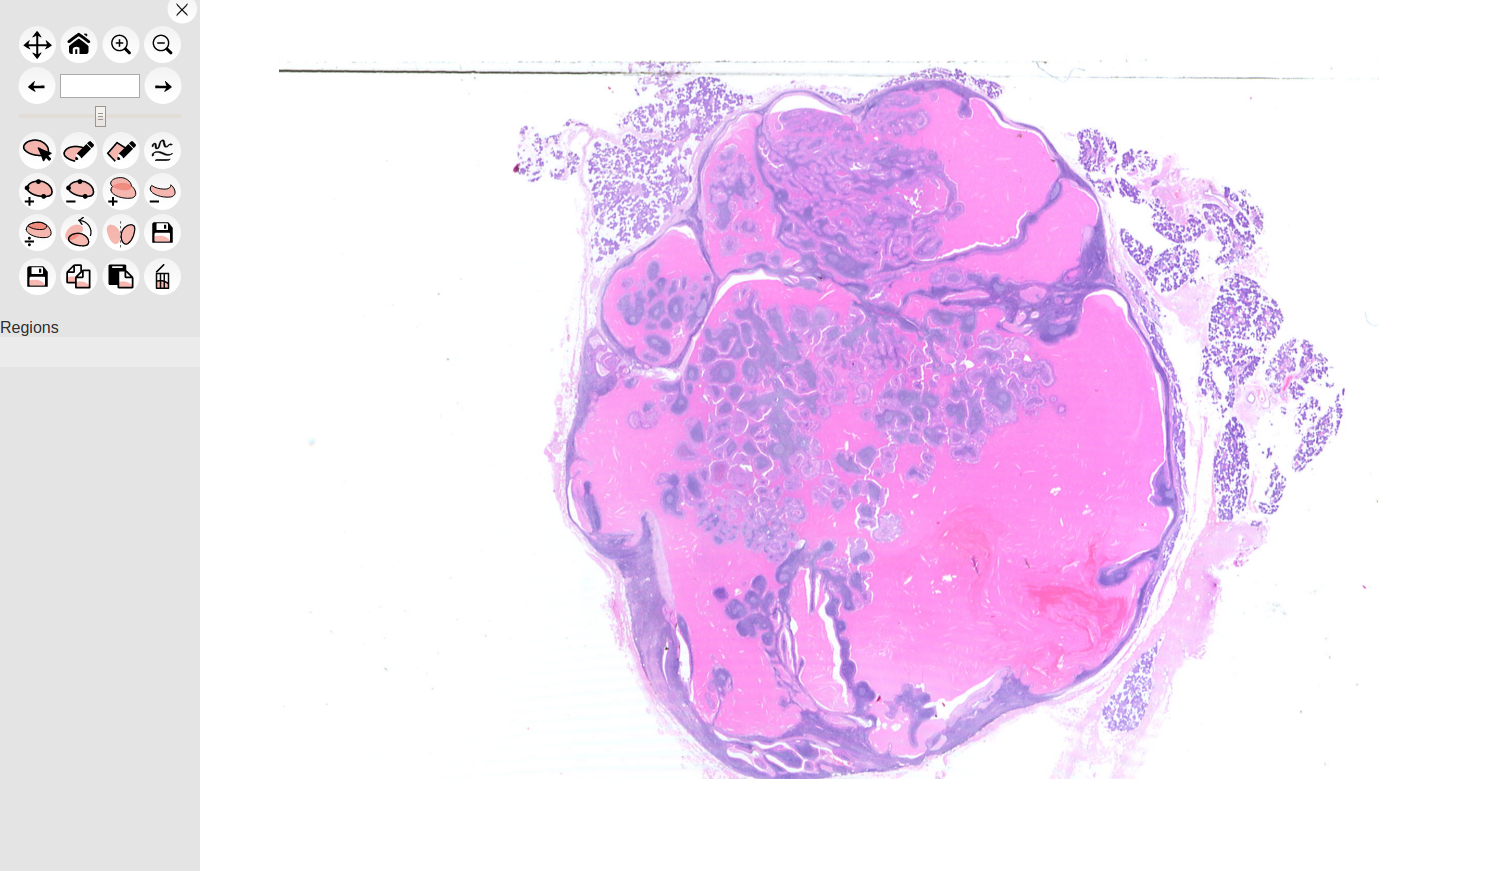
\includegraphics[scale=0.2]{img/microdrawUI.png}
		\caption{Microdraw GUI with opened WSI}
		\label{fig4_microdrawUI}
	\end{center}
\end{figure}

MicroDraw is a web application to view and annotate \emph{"high resolution histology data"}\cite{web:microdraw2}. The visualization is based on \emph{OpenSeadragon} (OSD)\nmc{OSD}{OpenSeadragon}\footnote{
	For more information visit OSDs repository on GitHub: \url{https://openseadragon.github.io/}.
}, another open source project. Annotations are made possible by the use of \emph{Paper.js}\footnote{See \url{http://paperjs.org/} for more information on Paper.js}. This delivers a baseline for the capabilities stated earlier in this subsection.

Each iteration of the ASV will be reviewed regarding its usability and functionality by a pathologist, thus adjusting it to its real life environment with each iteration.


\section{Annotation Service Server Implementation}
The ASS is a local server, implemented in python (\emph{\textbf{as{\textunderscore}server.py}}). It offers a RESTful styled API for communication (see subsection \ref{sec4_api}). To improve functionality, the following frameworks were used:

\begin{itemize}
	\item Flask (see subsection \ref{sec4_flask})
	\item OpenSlide Python (see subsection \ref{sec4_openslide})
\end{itemize}

All code snippets in the following subsections have been taken from \emph{\textbf{as{\textunderscore} server.py}}. A detailed documentation of the individual functions can be found in appendix \ref{sec_B1}.


\subsection{Flask}
\label{sec4_flask}
To give ASS its server capabilities, Flask was used\footnote{
	See Flasks homepage for additional information: \url{http://flask.pocoo.org/}
}. It provides a built-in development server, integrated unit testing, RESTful request dispatching and is Web Server Gateway Interface\footnote{
		The WSGI is a standard interface for the communication between web servers and web applications or frameworks in python. The interface has a server and application side. Basically, the server side invokes a callable object that is provided by the application side. The specifics of providing this object are up to the individual server\cite{Brandl16}.
} (WSGI)\nmc{WSGI}{Web Server Gateway Interface} compliant\cite{web:flask}.

Flask's so called \emph{route() decorator} provides a simple way to build a RESTful API for server client communication:

\begin{lstlisting}[language=Python, frame=single]
@app.route('/loadJson')
def loadJson(): 
	...

@app.route('/createDictionary')
def createDictionary():
	...

@app.route('/getDictionaries')
def getDictionaries():
	...
	
@app.route("/runSegmentation")
def runSegmentation():
	...
\end{lstlisting}

Decorating a function with \texttt{@app.route([URL])} will bind it to the supplied URL. When the client requests that bound URL, the server will call the decorated function\cite{web:flask}. The code snippet above shows exemplary how to use decorators.

A bound URL can also contain variable sections, which are marked as \emph{{\textless}variable name{\textgreater}}. Optionally, a converter can by used to only accept variables of a certain type. This becomes possible by specifying the converter in front of the variable: \emph{{\textless}converter:variable name{\textgreater}}\cite{web:flask}. The following code snippet shows possible examples for URLs with variables (see tab. \ref{tab4_converter} for a list of available converters):

\begin{lstlisting}[language=Python, frame=single]
@app.route('/wsi/<path:file_path>.dzi')
def index_dzi(file_path):
	...

@app.route('/wsi/<path:file_path>')
def index_wsi(file_path):
	...

@app.route('/<slug>.dzi')
def dzi(slug):
	...

@app.route('/<slug>_files/<int:level>/
<int:col>_<int:row>.<format>')
def tile(slug, level, col, row, format):
	...
\end{lstlisting}

To bind a URL with one or more variables, the corresponding function must be parameterized with same variables (compare line 1 and 2 or 13 - 14 and 15)\cite{web:flask}.

\begin{table}[H]
	\begin{center}
		\begin{tabular}{| l | l |}
			\hline
			\textbf{name} & \textbf{accepted input}\\ \hline
			string & any text without a slash (default)\\ \hline
			int & integer values\\ \hline
			float & floating point values\\ \hline
			path & like string, but also accepts slashes \\ \hline
			any & matches one of the items provided\\ \hline
			uuid & UUID strings\\ \hline
		\end{tabular}
		\caption{Available converters in Flask (source: \cite{web:flask})}
		\label{tab4_converter}
	\end{center}
\end{table}

HTTP knows different methods for accessing URLs (such as GET or POST)\cite{web:w3c}]. Flask will answer only GET requests by default. Any other method is answered with a "405 Method not allowed" HTTP status code\cite{web:flask}. This can be changed by adding the \emph{methods} argument to the decorator:

\begin{lstlisting}[language=Python, frame=single]
@app.route('/saveJson', methods=['POST'])
def saveJson():
	...
\end{lstlisting}

Tab. \ref{tab4_flaskBindigns} states a number of URLs, that have been bound to a corresponding function. For a detailed documentation of the individual functions, consult appendix \ref{sec_B1}.

\begin{table}[H]
	\begin{center}
		\begin{tabular}{| p{6.5cm} | p{3.5cm} |}
			\hline
			\textbf{URL} & \textbf{function}\\ \hline
			/wsi/{\textless}path:file{\textunderscore}path{\textgreater}.dzi & \texttt{index{\textunderscore}dzi(file{\textunderscore}path)}\\ \hline
			/wsi/{\textless}path:file{\textunderscore}path{\textgreater} & \texttt{index{\textunderscore}wsi(file{\textunderscore}path)}\\ \hline	
			/{\textless}slug{\textgreater}.dzi & \texttt{dzi(slug)}\\ \hline
			/{\textless}slug{\textgreater}{\textunderscore}files/{\textless}int:level{\textgreater}{\textunderscore}{\textless}int:col{\textgreater}{\textunderscore} {\textless}int:row{\textgreater}.{\textless}format{\textgreater} & \texttt{tile(slug, level, col, row, format)}\\ \hline
			/saveJson & \texttt{saveJson()}\\ \hline
			/loadJson & \texttt{loadJson()}\\ \hline
			/createDictionary & \texttt{createDictionary()}\\ \hline
			/getDictionaries & \texttt{getDictionaries()}\\ \hline
			/runSementation & \texttt{runSegmentation()}\\ \hline
		\end{tabular}
		\caption{ASS' URL-function binding overview}
		\label{tab4_flaskBindigns}
	\end{center}
\end{table}

\subsection{OpenSlide Python}
\label{sec4_openslide}
To read a WSI, ASS uses OpenSlide Python, which is a python interface to the OpenSlide C library. Besides providing an interface to read a WSI, it offers a DZI wrapper\cite{web:openslide}, called \emph{DeepZoomGenerator} (DZG)\nmc{DZG}{DeepZoomGenerator}. The DZG can be used to create Deep Zoom tiles on demand. The following formats are supported by OpenSlide\cite{web:openslide}:

\begin{itemize}
	\item BIF
	\item NDPI
	\item MRXS
	\item SCN
	\item SVS
	\item SVSLIDE
	\item TIF
	\item TIFF
	\item VMS
	\item VMU
\end{itemize}

This list is identical to the list of image formats supported by the CS (compare chapter \ref{sec3_cs}. This is due to the fact that \emph{VIPS} uses OpenSlide to read WSIs as well\cite{web:vips}.

OpenSlide can read a proprietary WSI as a so called \emph{OpenSlide} object (see line 4):

\begin{lstlisting}[language=python, frame=single]
from openslide import open_slide
from openslide.deepzoom import DeepZoomGenerator

slide = open_slide(slide path)
dzg = DeepZoomGenerator(slide[, tile_size, overlap, limit_bounds])
\end{lstlisting}

An OpenSlide object offers methods to access available metadata, image tiles, the thumbnail image and associated images, if available\footnote{
	See the OpenSlide documentation for further information: \url{http://openslide.org/api/python/}
} The OpenSlide object can be wrapped with a DZG to enable DZI support (see line 5)\cite{web:openslide}. A number of optional parameters can be passed into the constructor as well (see tab \ref{tab4_DZGparam} for parameters and their default values).

\begin{table}[H]
	\begin{center}
		\begin{tabular}{| p{2.5cm} | p{2cm} | p{5.5cm} |}
			\hline
			\textbf{parameter} & \textbf{type} & \textbf{description (default value)}\\ \hline
			osr & OpenSlide, ImageSlide & the slide object (mandatory)
			\\ \hline
			tile{\textunderscore}size & integer & the width and height of a single tile (254)\\ \hline
			overlap & integer & the number of extra pixels to add to each interior edge of a tile (1)\\ \hline
			limit{\textunderscore}bounds & boolean & true to render only the non-empty slide region (false)\\ \hline
		\end{tabular}
		\caption{DZG parameters (source: \cite{web:openslide})}
		\label{tab4_DZGparam}
	\end{center}
\end{table}

The DZG\footnote{
	For an in-depth list of functions, see \url{http://openslide.org/api/python/}
} generates all data necessary, to work with a proprietary WSI as if it would be a DZI\cite{web:openslide}. Of special importance are the \texttt{get{\textunderscore}dzi(format)} and \texttt{get{\textunderscore}tile(level, address)} functions.

\texttt{get{\textunderscore}dzi(format)} generates a string containing the complete metadata of a DZI XML file\footnote{
	Compare subsection \ref{sec2_openFormats} - Deep Zoom Images
}. The parameter (format) specifies the format (PNG or JPEG) of the individual Deep Zoom tiles.

\texttt{get{\textunderscore}tile(level, address)} returns an image of the tile corresponding to the provided parameter values (see tab. \ref{tab4_getTileParams}). The tiles are returned either as PNG or JPEG, depending on which format was chosen for \texttt{get{\textunderscore}dzi(format)}, 

\begin{table}[H]
	\begin{center}
		\begin{tabular}{| p{1.5cm} | p{1.5cm} | p{7cm} |}
			\hline
			\textbf{name} & \textbf{type} & \textbf{description}\\ \hline
			level & integer & the DZI level to get the tile from \\ \hline
			address & tuple & the address of the tile within the level as a (column, row) tuple\\ \hline
		\end{tabular}
		\caption{Description of \texttt{get{\textunderscore}tile(level, address)} parameters (source: \cite{web:openslide})}
		\label{tab4_getTileParams}
	\end{center}
\end{table}

The use of the DZG enables ASS to create DZI metadata and Deep Zoom tiles from proprietary WSI files on demand.


\subsection{Setup}
\label{sec4_setup}
To provide static files to Flask a \emph{static/} directory must be present at the root level of the ASS. This directory contains the CSS, JavaScript, dictionary, configuration and WSI files. To make a WSI accessible to the ASV, it must be placed in \emph{static/wsi/}. From there, the file path is arbitrary.

To provide a segmentation script, it must be placed in \emph{static/segmentation}. Furthermore, the name of the script must be adjusted in the configuration file (\emph{"segmentationScript"} in \emph{configuration.json}, see tab. \ref{tab4_assConfig} for a list of all configurable parameters). 

\begin{table}[H]
	\begin{center}
		\begin{tabular}{| p{3cm} | p{5.5cm} | p{2cm} |}
			\hline
			\textbf{parameter} & \textbf{description} & \textbf{standard}\\ \hline
			defaultFillAlpha & Default alpha value for regions & 0.5\\ \hline
			defaultStrokeColor & Default color for region strokes & black \\ \hline
			defaultStrokeWidth & Default width for region strokes & 1 \\ \hline
			dictionary & Name of currently active dictionary & example.json\\ \hline
			hideToolbar & Hide toolbar when ASV is rendered & false\\ \hline
			segmentationScript & Script used for segmentation of POIs & opencv.py\\ \hline
		\end{tabular}
		\caption{Configurable parameters in configuration.json}
		\label{tab4_assConfig}
	\end{center}
\end{table}

The ASS can be started from a terminal through the use of a python interpreter:
\begin{lstlisting}
$ python as_server.py
\end{lstlisting}

Alternatively, python's -m switch can be used:
\begin{lstlisting}
$ export FLASK_APP=as_server.py
$ python python -m flask run
\end{lstlisting}

When started, the server will listen on 127.0.0.1:5000 by default. Another port (-p, --port) or IP address (-l, --listen) can be specified when starting the ASS. Additionally, DZG-related parameters can be changed (see tab. \ref{tab4_assParams}).

\begin{table}[H]
	\begin{center}
		\begin{tabular}{| l | l | r |}
			\hline
			\textbf{parameter} & \textbf{description} & \textbf{default}\\ \hline
			-B, --ignore-bounds & render only the non-empty slide region & false\\ \hline
			-e, --overlap & set overlap between adjacent tiles in pixels & 0 \\ \hline
			-f, --format & set tile format (PNG or JPEG) & JPEG \\ \hline
			-l, --listen & set IP address to listen to & 127.0.0.1\\ \hline
			-p, --port & set port to listen to & 5000\\ \hline
			-Q, --quality & set JPEG compression quality in \% & 100\\ \hline
			-s, --size & set tile size & 256\\ \hline
		\end{tabular}
		\caption{Parameters for as{\textunderscore}server.py}
		\label{tab4_assParams}
	\end{center}
\end{table}

To retrieve a WSI from the ASS, the URL must be pointed to it in the following manner: \emph{http://[host]:[port]/wsi/[file path]} (see fig. \ref{fig4_wsiUrl} for an example).

\begin{figure}[H]
	\begin{center}
		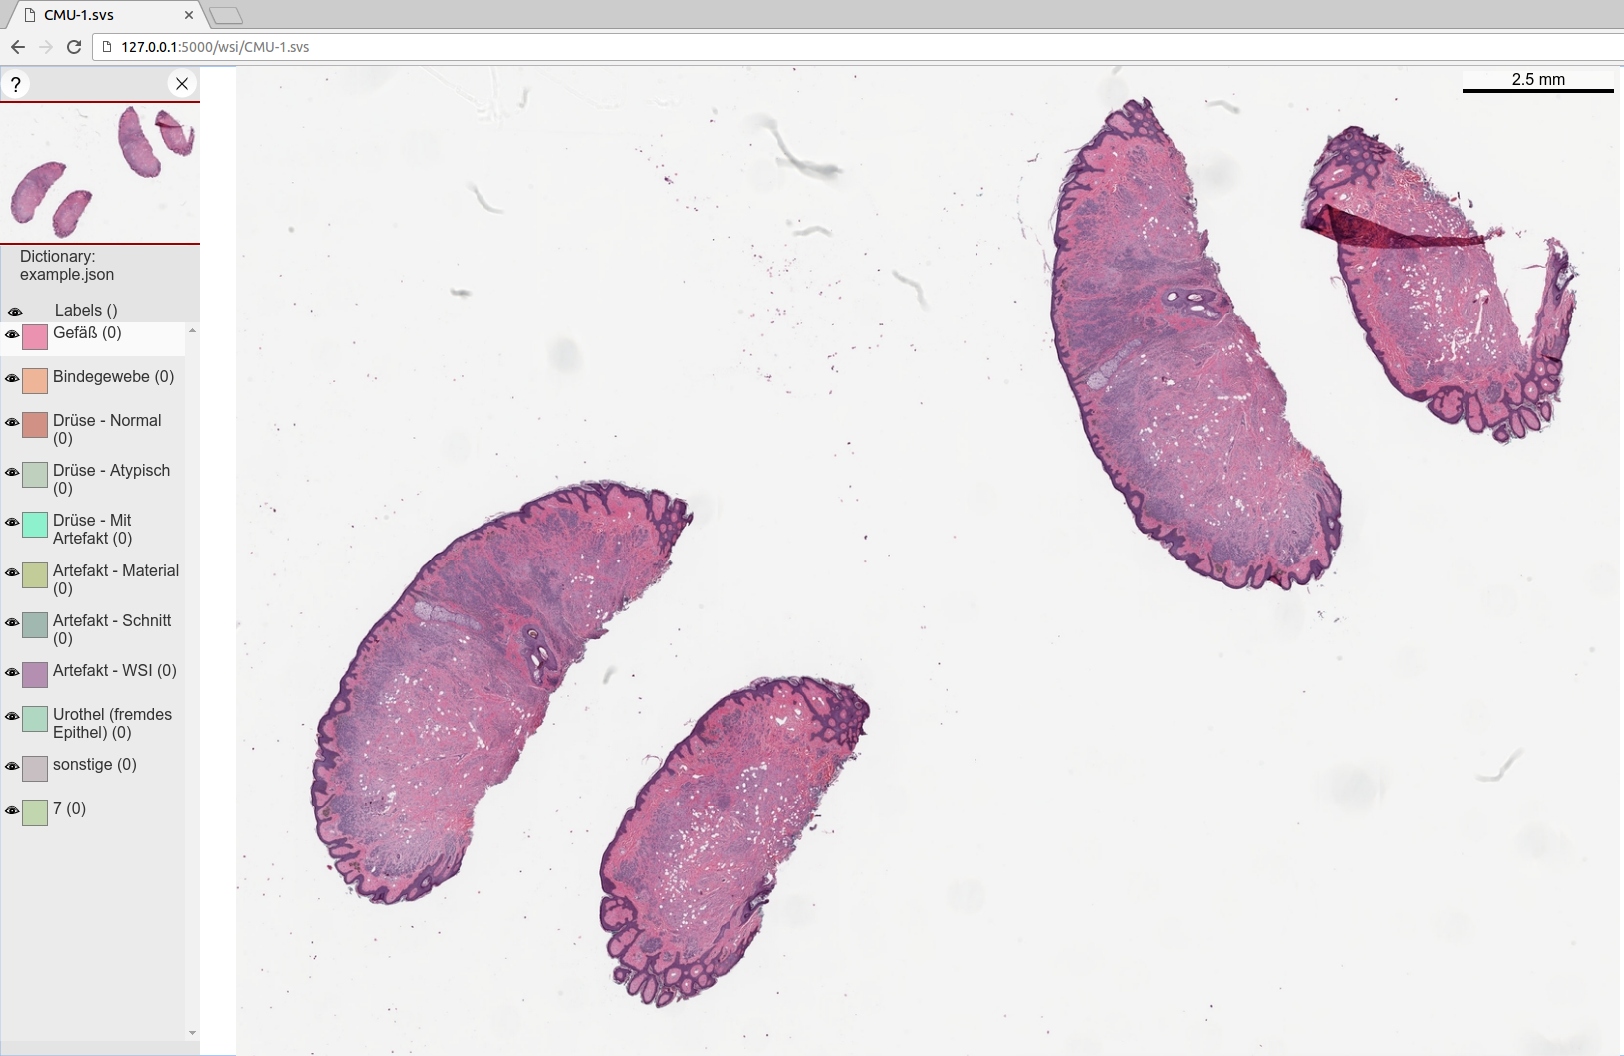
\includegraphics[scale=0.2]{img/wsiUrl.png}
		\caption{Example URL to retrieve WSI (\url{http://127.0.0.1:5000/wsi/CMU-1.svs)}
		\label{fig4_wsiUrl}; WSI source: OpenSlides freely distributable test data (see appendix \ref{sec_A1})}
	\end{center}
\end{figure}


\subsection{RESTful API}
\label{sec4_api}
The ASS provides a RESTful API. This was realized with Flasks route() decorators\footnote{See subsection \ref{sec4_flask}} (compare tab. \ref{tab4_flaskBindigns} for a list of corresponding functions). The listing below gives an overview over the URLs offered by the API:

\begin{enumerate}[(1) -]
	\item\textbf{/wsi/[file path].dzi\\
	method:} GET\\
	Requests an ASV to view the requested DZI. [file path] must point to a valid DZI, otherwise a "404 Not Found" HTTP status code is returned.\\
	\emph{Returns} either a rendered ASV, which requests the DZI at [file path] or "404 Not Found"
	
	\item \textbf{/wsi/[file path]\\
	method:} GET\\
	Works similar to (1), except that the requested image is a proprietary WSI instead of a DZI. Thus, a DZG is created to wrap the slide.\\
	\emph{Returns} a specifically generated URL (\emph{[slug].dzi}).
	
	\item \textbf{/[slug].dzi\\
	method:} GET\\
	Requests the DZI metadata of [slug] from the DZG. A corresponding DZG will only exist, if (2) was called beforehand. Never call this function manually, to ensure a safe execution of the related commands. The ASV will call this function automatically.\\
	\emph{Returns} the DZI metadata generated by the DZG or "404 Not Found" if no corresponding DZG was found.
	
	\item \textbf{/[slug]{\textunderscore}files/[level]{\textunderscore}[col]{\textunderscore}[row].[format]\\
	method:} GET\\
	Requests the Deep Zoom tile [col]{\textunderscore}[row].[format] in [level] from the DZG. As with (3), do not call this function manually. The ASV will call it automatically to retrieve the image tiles needed.\\
	\emph{Returns} the image tile in the specified level at the requested position or "404 Not Found" if no image tile could be generated.
	
	\item \textbf{/saveJson\\
	method:} POST\\
	Post request that saves the provided JSON data in the provided JSON file. Creates a new one, if it does not exist. The posted data must look like the following:
	\begin{lstlisting}
	{
		"file":"[file name]",
		"content":"[json content]"
	}
	\end{lstlisting}
		
	\item \textbf{/loadJson?src=[source]\\
	method:} GET\\
	Loads the JSON file specified in [source].\\
	\emph{Returns} the JSON data if a file was found, an empty JSON map ("[]") otherwise.
	
	\item \textbf{/createDictionary?name=[name]\\
	method:} GET\\
	Requests the creation of a new, empty dictionary. The file will be called [name]. The ASV adds a ".json" if necessary. A manual call of this functions makes an added ".json" necessary. Otherwise, a text file will be created.\\
	\emph{Returns} the name and path to the new dictionary as json:
	\begin{lstlisting}
	{
		"name":"[name]",
		"path":"[dictionary path]"
	}
	\end{lstlisting}
	or "error" if [name] is already taken by another dictionary.\clearpage
	
	\item \textbf{/getDictionaries\\
	method:} GET\\
	Requests a list of files contained in the \emph{dictionaries} folder.\\
	\emph{Returns} a list with the file names, or "-1" if no dictionaries are present.
	
	\item \textbf{/runSegmentation?x=[x]\&y=[y]\\
		method:} GET\\
	Requests the invocation of the segmentation script provided in the configuration file. The coordinates of the POI are passed as URL arguments and will be handed down to the segmentation script.\\
	\emph{Returns} a list of 2D coordinates, describing the contour around the POI, or a "404 Not Found" HTTP status code if no script was provided or the provided script was not found.
\end{enumerate}


% python web server, flask, openslide, java script, html5, css, jquery
\section{Annotation Service Viewer Implementation}

The ASV is a browser application based on the MicroDraw open source project. It provides a client with a WSI viewer with annotation capabilities (see subsection \ref{sec4_asvPart}). It is implemented using JavaScript, HTML5 and CSS. The following frameworks were used to add additional functionality:

\begin{itemize}
	\item jQuery
	\item OSD
	\item Paper.js
\end{itemize}

The ASV consists of the following files:

\begin{itemize}
	\item \emph{as{\textunderscore}viewer.html} (template/)
	\item \emph{as{\textunderscore}viewer.js} (static/lib/)
	\item \emph{as{\textunderscore}viewer.css} (static/css/)
	\item \emph{style.css} (static/css/)
\end{itemize}

A documentation of the individual functions of the ASV JavaScript (as{\textunderscore}server.js) can be found in appendix \ref{sec_B2}.

\subsection{Frameworks}
The ASV uses jQuery, OSD and Paper.js for additional functionality.

jQuery is a common JavaScript library, that offers an API to handle HTML document traversal and manipulation, event handling, animation and AJAX\footnote{
	Asynchronous JavaScript and XML (AJAX)\nmc{AJAX}{Asynchronous JavaScript and XML} is a group of technologies which enable a client to make asynchronous web requests\cite{Ullman07}.
} requests\cite{web:jquery}. It is also supported by all common web browsers\cite{web:jqueryBS}. The ASV uses jQuery especially for its HTML document traversal and manipulation capabilities, as well as its AJAX support.

See the corresponding subsections for OSD and Paper.js.

\subsubsection{OpenSeadragon}
OSD is used by the ASV to show a WSI. It is a JavaScript based, open source web application to serve a viewer for \emph{"high-resolution zoomable images"}\cite{web:openseadragon}. It supports the following image formats:

\begin{itemize}
	\item DZI
	\item IIIF
	\item OSM
	\item TMS
\end{itemize}

Furthermore, custom tile sources can be added to support other image formats as well. Since the ASS is capable of delivering every WSI as DZI, no custom tile source implementation is necessary for proprietary WSIs\footnote{
	Compare subsection \ref{sec2_openFormats}.
}.

The ASV defines a \textless{div}{\textgreater} in its HTML file, which will be used to hold the OSD viewer (OSDV)\nmc{OSDV}{OpenSeadragon Viewer}:
\begin{lstlisting}[title=as{\textunderscore}viewer.html, frame=single, language=html]
<!-- OpenSeadragon viewer -->
<div id="openseadragon1" style="width:vh;height:hh"></div>
\end{lstlisting}

The OSDV is then created in the ASV's JavaScript file:
\begin{lstlisting}[title=as{\textunderscore}viewer.js, frame=single, language=JavaScript]
 // create image viewer
 viewer = OpenSeadragon({
	 id: "openseadragon1",
	 prefixUrl: staticPath + "/lib/openseadragon/images/",
	 showReferenceStrip: false,
	 showNavigator: true,
	 sequenceMode: false,
	 navigatorId:"myNavigator",
	 zoomPerClick: 1,
 });
\end{lstlisting}

The relation between \textless{div}{\textgreater} and OSDV is created through the \emph{id} parameter (line 3). Tab. \ref{tab4_osdvParams} states a description of every parameter used in the above constructor\footnote{
	See \url{https://openseadragon.github.io/docs/OpenSeadragon.html\#.Options} for an in-depth documentation of every parameter available.
}.
\begin{table}[H]
	\begin{center}
		\begin{tabular}{| p{3.5cm} | p{6.5cm} |}
			\hline
			\textbf{parameter} & \textbf{description}\\ \hline
			id & Id of the element to append the viewer's container element to.\\ \hline
			prefixUrl & Prepends the provided prefixUrl to the path for the OSDVs internal images.\\ \hline
			showReferenceStrip & If true, display a scrolling strip of image thumbnails for navigating through the images.\\ \hline
			showNavigator & Makes the navigator minimap visible if true. \\ \hline
			sequenceMode & Set to true to view a sequence of images.\\ \hline
			navigatorId & The ID of a div to hold the navigator minimap.\\ \hline
			zoomPerClick & The distance to zoom in on every mouse click. Setting it to 1.0 disables the feature.\\ \hline
		\end{tabular}
		\caption{Overview of used options in OSDV constructor (source: \cite{web:openseadragon})}
		\label{tab4_osdvParams}
	\end{center}
\end{table}

Since drawing paths and managing regions involves clicking onto the corresponding ROIs on the WSI, the zoomPerClick function must be disabled. Otherwise it will be called after each of those interactions, which is highly disorienting.

The OSDV provides an \texttt{open(tileSources)} function, which is used to open a DZI's tiles\footnote{
	DZI, as well as all other image formats, supported by the OSDV implement a tiled image pyramid scheme (see \ref{sec:dicomSupplement}). Thus, a number of images must be opened.
}. The tileSources are provided as URL to the DZI's metadata file by the ASS (either "/static/wsi/[file].dzi" (natural DZI) or "/static/slide.dzi" (artificial DZI from the DZG\footnote{
	Compare subsection \ref{sec4_openslide}.
})). Based on the URL extension (always \emph{".dzi"} in this AS' scope), the OSDV selects an appropriate \emph{TileSource} interface to access the individual tiles and levels of the provided image format.

A scalebar is added to the OSDV to support the assessment of ROIs:

\begin{lstlisting}[title=as{\textunderscore}viewer.js, frame=single, language=JavaScript]
var mpp = 0;
if(slide.mpp) {
	ppm = slide.mpp > 0 ? (1e6 / slide.mpp) : 0
}

viewer.scalebar({
	type: OpenSeadragon.ScalebarType.MICROSCOPE,
	minWidth:'150px',
	pixelsPerMeter:ppm,
	color:'black',
	fontColor:'black',
	backgroundColor:"rgba(255,255,255,0.5)",
	barThickness:4,
	location: OpenSeadragon.ScalebarLocation.TOP_RIGHT,
	xOffset:5,
	yOffset:5
});
\end{lstlisting}

The scale is $pixels/{\mu}m$. Since the ASS only delivers MPP (which is ${\mu}m/pixel)$ and the OSDV's scalebar expects $pixels/m$ (\emph{PPM}), a conversion is necessary:
\begin{equation}\label{eq:ppm}
	PPM = \frac{10^6}{MPP}
\end{equation}

Eq. \ref{eq:ppm} can be seen in line 3 of the code snippet above.  If no valid input is provided from the ASS (that is: when no value was specified for MPP in the WSI's metadata), PPM will be set to 0. If the pixelPerMeter parameter of the scalebar equals 0 it is automatically hidden\cite{web:openseadragon}. The options in line 7 - 16 concern the styling of the scalebar (such as color, position and size).

When navigating through the tiles and layers of the OSDV's tile source, it will automatically request the tiles needed for the current view from the ASS via HTTP GET\cite{web:openseadragon}.


\subsubsection{Paper.js}
The ASV utilizes Paper.js to create a region's path. Paper.js is an \emph{"open source vector graphics scripting framework"}, running on top of the HTML5 canvas\cite{web:paper}. It offers an API to create and manage vector graphics and bezier curves\footnote{
	A \emph{bezier curve} is a parametric curve, frequently used in computer graphics\cite{Strang03}.
}. Additionally, it offers vector relevant entities, such as \emph{point}, \emph{size} and \emph{rectangle} objects and enables the drawing of finely grained paths.

When the OSDV opens an image, a so called \emph{annotation overlay} (AO)\nmc{AO}{Annotation Overlay} is created:
\begin{lstlisting}[title=Excerpt from \texttt{initAnnotationService()} in as{\textunderscore}viewer.js, frame=single, language=JavaScript]
viewer.addHandler('open',function(){
	initAnnotationOverlay();
	[...]
}
\end{lstlisting}

The AO is a canvas which is placed above the OSDV. On it, paths can be drawn, which will be used to enclose an ROI. The AO is initialized in \texttt{initAnnotationOverlay()} (see line 3 in the code snippet above). Once created, the AO is resized to fit the opened WSI in height and width. This only happens when initializing the canvas. Therefore the AO will have (and keep) the dimensions of the level the WSI was opened in.

This leads to issues when zooming in and out onthe OSDV (and consequently changing the level of the tile source). To counteract this, the AO is stretched to fit the new dimensions of the WSI's currently viewed layer. This leads to the problem of having different pixel densities in AO and OSDV.

The AO is of very fine granularity and, when added programmatically, can create path segments within the decimals of a single pixel\cite{web:paper}. In drawing mode however, segments are only added between whole pixels, making it impossible to draw regions in high zoom levels. Since both, AO and OSDV, calculate clicked pixel positions from the clicked pixel in the browser\cite{web:openseadragon},\cite{web:paper}, a conversion is possible. Two conversion functions haven been implemented:
\begin{enumerate}[(1)]
	\item\label{item_AOtoIC} AO coordinate $\rightarrow$ image coordinate
	\item\label{item_ICtoAO} image coordinate $\rightarrow$ AO coordinate
\end{enumerate}

The corresponding functions are \texttt{convertPathToImgCoordinates(point)} for (\ref{item_AOtoIC}) and \texttt{convertImgToPathCoordinates(point)} for (\ref{item_ICtoAO}). The following code snippet shows their implementation:

\begin{lstlisting}[title=as{\textunderscore}viewer.js, frame=single, language=JavaScript]
function convertPathToImgCoordinates(point) {
	// convert to screen coordinates
	var screenCoords = paper.view.projectToView(point);
	// convert to viewport coordinates
	var viewportCoords = viewer.viewport.pointFromPixel(new OpenSeadragon.Point(screenCoords.x, screenCoords.y));
	// convert to image coordinates
	var imgCoords = viewer.viewport.viewportToImageCoordinates(viewportCoords);
	return imgCoords;
}

function convertImgToPathCoordinates(point) {
	// convert to viewport coordinates
	var viewportCoords = viewer.viewport.imageToViewportCoordinates(point);
	// convert to screen coordinates
	var pixel = viewer.viewport.pixelFromPoint(viewportCoords);
	// convert to project coordinates
	var projectCoords = paper.view.viewToProject(pixel);
	return projectCoords;
}
\end{lstlisting}

\texttt{convertPathToImgCoordinates(point)} receives a point that is in the AO coordinate system and turns it into a screen coordinate (line 3). The screen coordinate is converted into a viewport coordinate\footnote{
	A viewport coordinate maps coordinates into values within the interval $[0, 100]$ for both dimensions, instead of using pixel coordinates\cite{web:openseadragon}.
} (line 5) from where it can be turned into an actual image coordinate (line 7).

\texttt{convertImgToPathCoordinates(point)} receives a point coordinate of the baseline image, which is turned into a viewport coordinate (line 13). The viewport coordinate is turned into a screen coordinate (line 15), to be turned into an AO coordinate from there (line 17).

Both of those functions need to work with the viewport coordinates to create a relation between the dimensions of the image and the current level.

\subsection{Definition: Region}
\subsection{GUI}
\subsection{Tools}